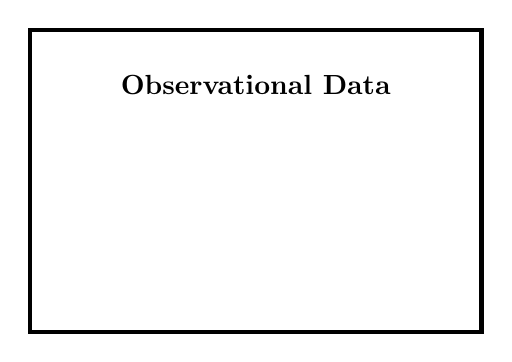
\begin{tikzpicture}[>=latex]
\usetikzlibrary{shapes,backgrounds,calc,arrows,positioning,arrows.meta}
\tikzset{>=stealth'}

\tikzstyle{bubble}=[draw, text centered, rounded corners, inner sep=1ex, thick]
\tikzstyle{cr}=[very thick]

% top left
\node(poc1)[draw, text centered, ultra thick, text width=5.5cm, text height=3.6cm] at (0.5,0.5) {};
\node(poc1t)[text centered, anchor=north] at ($(poc1.north)!{(1/8)}!(poc1.south)$) {\textbf{Observational Data}};

\end{tikzpicture}